\chapter{Introducción}
	
Este primer capítulo describe de forma general la información principal y relevante para poder comprender el funcionamiento del producto actual LUCA, así como los objetivos del proyecto a desarrollar junto con la explicación y motivación del mismo.
	
\section{Introducción}
	
	
En los últimos años, el volumen de datos que una empresa o entidad necesita o es capaz de gestionar o manipular ha aumentado de forma vertiginosa. Estos datos se almacenan en fuentes de diversos tipos, abarcando elementos tan dispares como bases de datos relacionales, hojas XML o repositorios FTP, a los cuales se accede mediante diferentes formas y lenguajes. Por tanto, un nuevo problema que debemos enfrentar, adicional al del volumen de datos a manipular, es que para acceder cierta información es necesario muchas veces establecer comunicaciones entre diferentes fuentes.

\vspace{5mm}
			
%%===================================================================%%
%% NOTE(Pablo): Meter aquí el ejemplo del resumen de nuevo, si se
%%              quiere más detallado
%%===================================================================%%

%% Init resumen

	 Como consecuencia de esta nueva situación, cuando un usuario	quiere obtener una información concreta cuyos datos residen en varios de estos
sistemas, necesita acceder a cada uno de estos sistemas, extraer de cada sistema la información que precisa, filtrarla y unificarla para finalmente	obtener los datos requeridos.

\vspace{5mm}

Por ejemplo, una tienda de electrodomésticos podría tener sistemas informáticos diferentes para el departamento de atención al cliente, para el departamento técnico de postventa y para el departamento de compras y adquisiciones.Por tanto, para conocer el estado actual de una reparación, podríamos necesitar:
\begin{itemize}
	\item  Acceder al primer sistema para obtener el identificador de la incidencia y en qué fase de su gestión se encuentra.
	\item  Comprobado que la incidencia está actualmente en reparación, recuperaríamos otro sistema el estado detallado de la reparación, comprobando que está a la espera de una pieza.
	\item Finalmente accederíamos al sistema de compra y adquisiciones para comprobar cuando está prevista la entrega de dicha pieza. Los sistemas de almacenamiento de la información pueden ser diversos, incluyendo desde un servicio web, una base de datos relacional, un repositorio de ficheros accesible vía FTP o una base de datos NoSQL.
\end{itemize}


\section{LUCA}

%% End resumen
			
Con el objetivo de facilitar este proceso de recuperación de información almacenada en sistemas y fuentes de datos hetereogéneas, dentro de la empresa CIC, se está desarrollando una aplicación denominada LUCA. Para facilitar este proceso de recuperación de información, LUCA proporciona un lenguaje común para todas las fuentes de datos a unificar, permitiendo al usuario abstraerse de los detalles de cada fuente.

\vspace{5mm}

%%===================================================================%%
%% NOTE(Pablo): Poner un ejemplo sencillo que muestre el
%%              funcionamiento de LUCA
%%===================================================================%%



%% Ejemplo Luca

A continuación se explica brevemente el funcionamiento de Luca con algunos ejemplo gráficos orientativos para ayudar a la comprensión del propio funcionamiento.

\vspace{5mm}

Para explicar el funcionamiento principal de dicho producto, se pretende describir el proceso de creación y ejecución de una consulta a un servicio REST.

\vspace{5mm}

En la vista inicial nos encontramos con una lista de consultas ya almacenadas, así como, una serie de filtros y opciones para la creación, ejecución y edición de consultas. Como se pretende explicar la creación y ejecución de una consulta, para avanzar en la vista se seleccionaría la creación de una nueva consulta.


\vspace{5mm}

A continuación, se muestra un ejemplo sobre un servicio REST, concretamente sobre el servicio REST de información de la flota de autobuses de Santander (TUS), donde tras introducir el identificador de una parada de autobús, se devolverá la información relativa a dicha parada, como es la localización.


	
	\begin{figure}[H]
		\centering
 		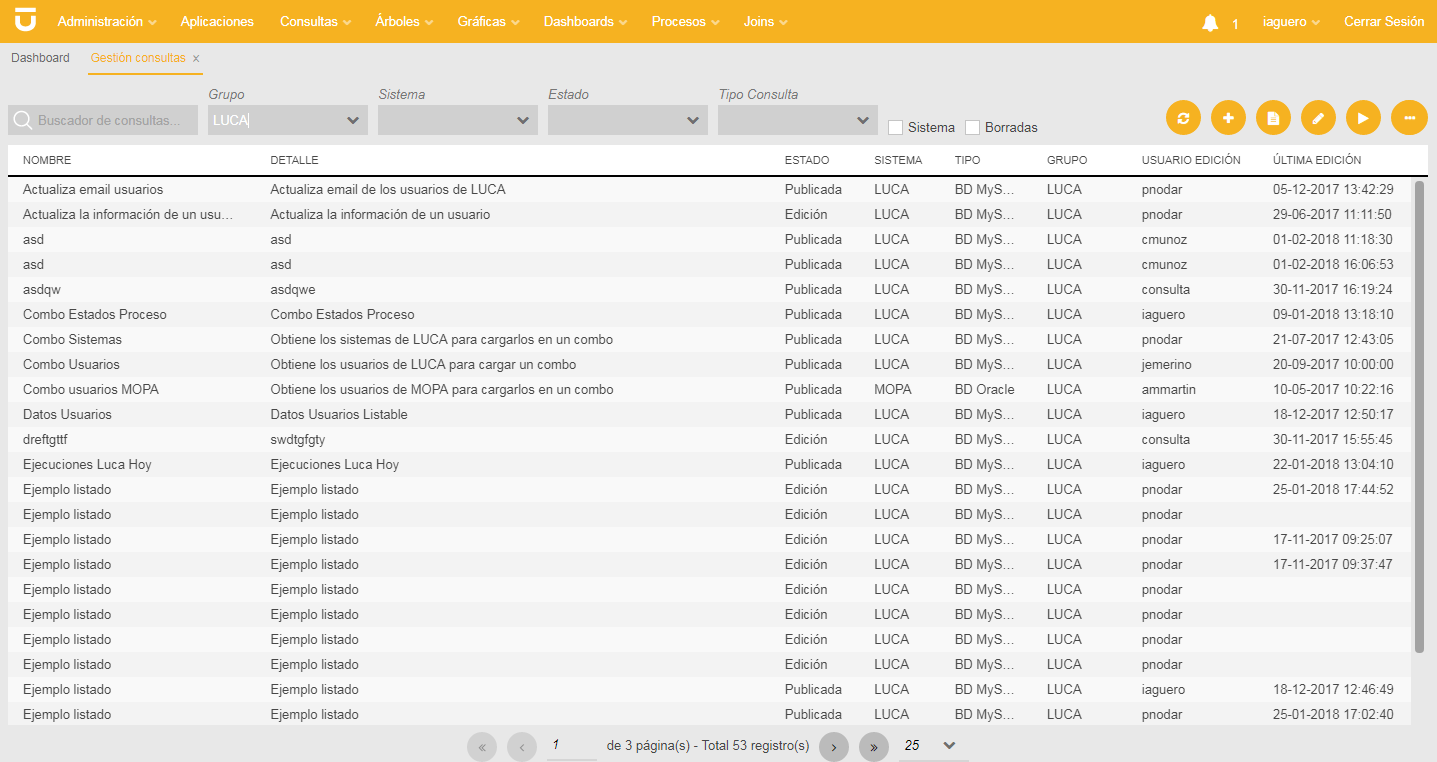
\includegraphics[scale=0.5]{capturasLuca/gestionConsultas.png}
		\caption{Vista de Gestión de Consultas}\label{fig:gestionConsulta}
	\end{figure}

Tras seleccionar la opción de creación de una nueva consulta, se muestra una vista en la que se permite agregar toda la información relativa a la consulta, como son las variables de entrada o de salida, o el tipo de salida que se desea recibir.

\vspace{5mm}

Una vez introducido el identificador de la parada, y seleccionado el botón de ejecución para llevar a cabo la ejecución de la consulta, se muestra el resultado de la consulta, el cuál puede ser visualizado de diferentes formas en función del recurso al que se llama.


	\begin{figure}[H]
		\centering
		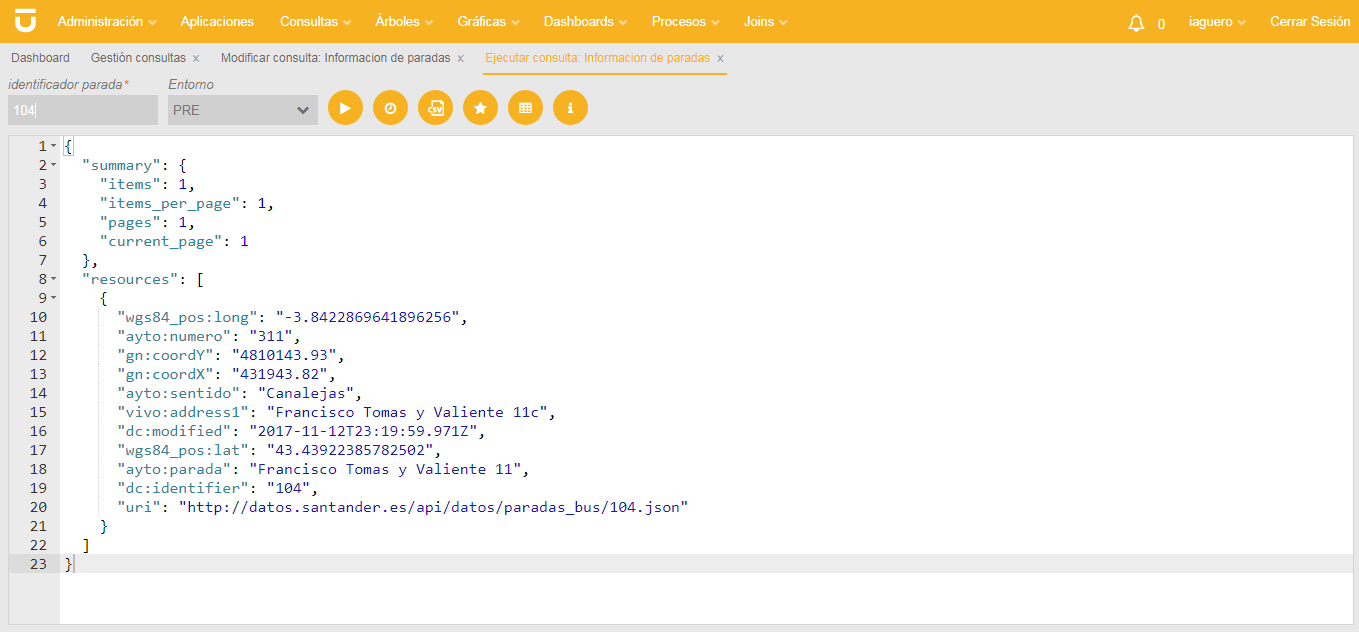
\includegraphics[scale=0.5]{capturasLuca/ejecucionConsulta.png}
		\caption{Vista de Ejecución de Consultas}\label{fig:ejecucionConsultas}
	\end{figure}


\vspace{5mm}


%% Fin ejemplo Luca

Actualmente LUCA proporciona mecanismos para permitir al usuario recuperar de manera uniforme información de diferentes fuentes de datos. No obstante, LUCA actualmente sólo es capaz recuperar información de una única fuente de datos a la vez. Por tanto, cuando es necesario combinar información procedente de distintas fuentes, el propio usuario es el que debe realizar dicho proceso de composición, ejecutando cada consulta a mano, y utilizando las salidas de cada una de ellas como las entradas de las siguientes.

\vspace{5mm}
			
%%===================================================================%%
%% NOTE(Pablo): Poner un ejemplo cómo es el proceso de composición
%%              a mano
%%===================================================================%%

Un ejemplo de dicho proceso de composición sería la necesidad de un dependiente de una tienda de electrodomésticos de obtener la edad de los usuarios que compraron lavadoras durante el mes pasado. Actualmente, los pasos o consecución de consultas que debería de realizar serían las siguientes:

\begin{itemize}
	\item  Primero necesitaría obtener el registro de compras del mes pasado del sistema.
	\item  Después, tras apuntarse dicho registro, tendría que, uno por uno, seleccionar los que se corresponden con lavadoras.
	\item Una vez que el usuario tiene las lavadoras compradas el mes pasado, éste tendría que recoger que usuarios han comprado las lavadoras.
	\item Por último, el usuario debería de buscar en el sistema cada usuario que ha realizado la compra, con el nombre obtenido previamente.
\end{itemize}

Se puede observar que el usuario tiene un engorroso desarrollo de acciones para poder obtener el resultado deseado.

\vspace{5mm}

%% Fin ejemplo composición

El objetivo de este proyecto es facilitar dicho proceso de composición al usuario mediante el desarrollo de un mecanismo gráfico para la especificación de estos procesos de composición de consultas.

\vspace{5mm}

%%===================================================================%%
%% NOTE(Pablo): Dar algunos detalles técnicos de cómo se pretente
%%              construir esto.
%%===================================================================%%
Para llevar a cabo esta tarea, se pretende realizar un sistema que permita visualmente utilizar las consultas ya almacenadas, para posteriormente relacionarlas entre sí mediante sus entradas y salidas y los tipos de las mismas. De esta forma, se podrá ejecutar automáticamente una cadena de consultas para obtener un resultado concreto, bajo un único concepto llamado Proceso.


\section{Ingeniería de Requisitos}

En esta sección se contará el proceso llevado a cabo para aprender o entender la estructuración y definición de requisitos de la actual LUCA, así como la propia descripción de los requisitos que serán necesarios para la implementación del proyecto a realizar.

\subsection{Proceso de integración en LUCA}

El primer paso llevado a cabo para la introducción en el producto de LUCA y entender así su funcionamiento, fue una reunión con el Jefe de Proyecto y con el Gerente para describir, analizar y explicar todos los aspectos de LUCA.

\subsection{Definición de Requisitos}

Una vez aclarados los términos del actual LUCA, se abordo el incremento que se quería llevar a cabo, del que parte este Trabajo de Fin de Grado. Se explicaron los términos de Proceso, variables de entradas y de salidas, consultas y demás.

\vspace{5mm}

Además de la explicación, se proporcionaron unos documentos técnicos tanto del componente gráfico del proceso como del incremento sobre LUCA. Estos documentos pueden encontrarse en el Anexo adjunto a la memoria.

\vspace{5mm}

Dado que la aplicación a construir es un incremento de un producto ya existente, no hace falta identificar la fuente de los requisitos ya que es el propio gerente o impulsor de dicho incremento el que actúa como stakeholder, junto con el jefe del proyecto los encargados de formar los objetivos conjuntos de la captura de información y de los propios requisitos.

\vspace{5mm}

Cabe explicar también, que este proyecto se funda en la implementación o desarrollo de dos componentes. El primero representa una herramienta focalizada en el ámbito gráfico, cuya función es la creación, borrado y actualización de elementos que constan de variables de entradas y salidas, en términos generales, manipulación gráfica de los elementos constituyentes del proyecto. El otro representa un proyecto incremento del actual producto LUCA, centrado en la gestión de los procesos, los cuales son creados a través de consultas y enlaces entre sus entradas y salidas.

\vspace{5mm}

Como ya se ha mencionado, en estos documentos se pueden encontrar los requisitos técnicos atribuidos al proyecto, pero, de forma resumida, se centran en tres pilares o requisitos principales:

\begin{itemize}
	\item  Concatenación de las consultas entre si pertenecientes a un mismo proceso.
	\item  Visualización del progreso de ejecución del proceso.
	\item Aplicar criterios de navegación a partir de los resultados de salidas.
\end{itemize}

La especificación de estos requisitos se encuentra en los documentos técnicos citados anteriormente.



\section{Arquitectura LUCA}

Esta sección se propone explicar y especificar la actual arquitectura de LUCA, así como, mostrar la integración con el componente o proyecto gráfico (Luca-Process), el cuál, a su vez, utiliza un componente javascript abstracto implementado con la librería javascript GO.JS.


\begin{figure}[H]
	\centering
	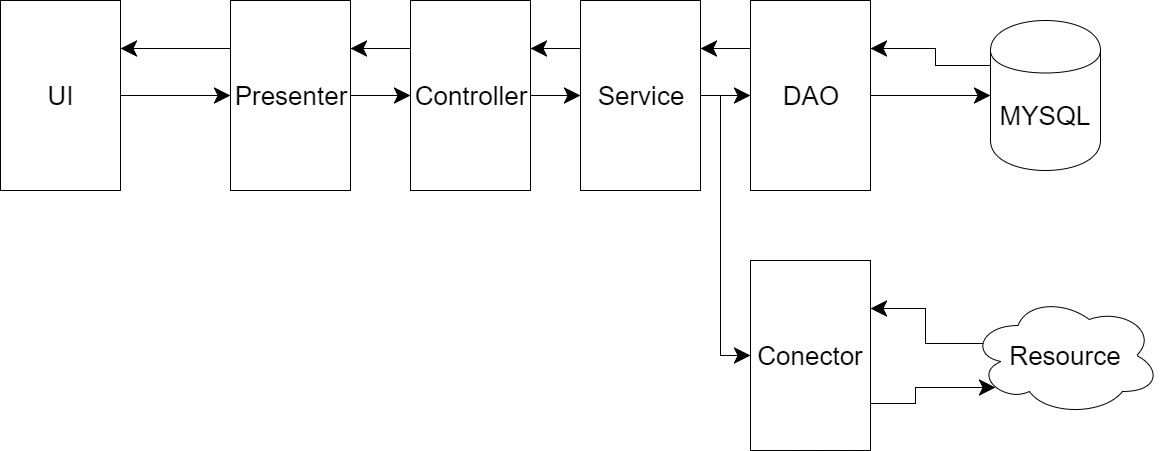
\includegraphics[scale=0.5]{funcionamientoLuca.png}
	\caption{Arquitectura de LUCA}\label{fig:funcionamientoLuca}
\end{figure}


Para comenzar, se explica a continuación la arquitectura de LUCA previa al incremento que se propone realizar.
En la figura superior podemos observar una arquitectura en tres capas bajo el patrón modelo-vista-presentador (MVP). Este patrón se caracteriza por separar de forma clara y concisa las vistas de la lógica de negocio.

\vspace{5mm}

En la arquitectura mostrada podemos observar, que la capa del presenter es la encargada de realizar la comunicación y control entre la vista y el modelo, y de albergar la gestión de eventos desde la vista.

\vspace{5mm}

Otro aspecto importante reside en la capa de servicio. Esta capa es la encargada de recibir los datos desde las diferentes fuentes de datos, ya sea de la base de datos de LUCA, o de un recurso externo de cualquier tipo (como por ejemplo la extracción de  información de un servicio REST, SOAP o de otra base de datos ajena).

\vspace{5mm}

Respecto a la arquitectura tras la integración de la nueva funcionalidad, la siguiente figura describe la diferencia respecto a la figura anterior:

\begin{figure}[H]
	\centering
	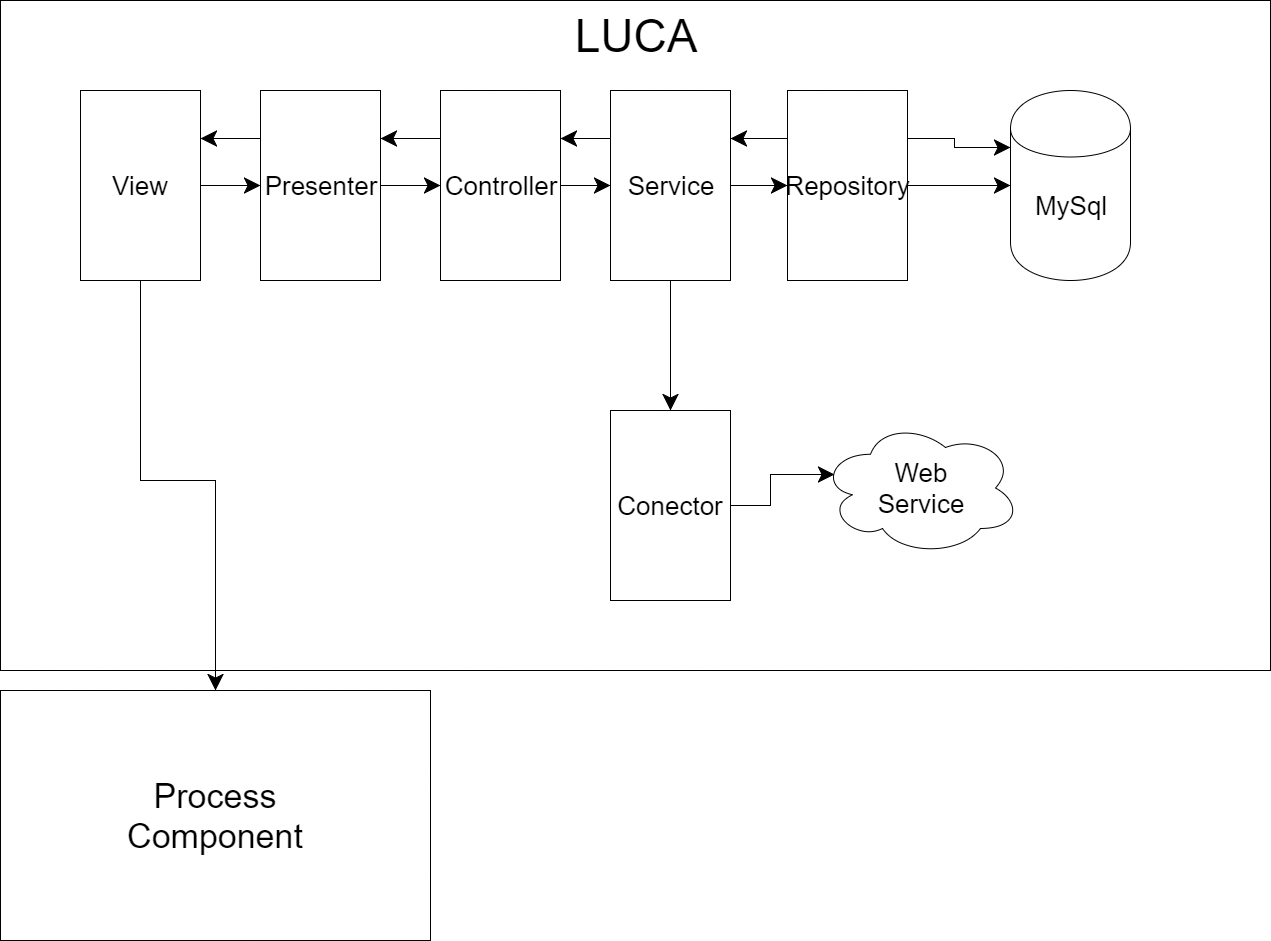
\includegraphics[scale=0.5]{arquitecturaLuca.png}
	\caption{Nueva Arquitectura de LUCA}\label{fig:arquitecturaLuca}
\end{figure}

Como se puede apreciar, la única diferencia reside en que en esta citada nueva funcionalidad se utiliza otro proyecto aparte, el cuál se encarga de forma exclusiva de proveer componentes de visualización para poder abordar la sintaxis de procesos y subprocesos que se enlazan entre sí mediante entradas y salidas.

\vspace{5mm}

A continuación se muestran dos apartados que describen el funcionamiento y arquitectura del conector de LUCA y del Process-Component.

\subsection{Arquitectura del Conector}


El conector de LUCA es un componente que se encarga de recibir o recoger los datos de los diferentes recursos albergados en las diferentes fuentes de datos externas. Puede ser de diferentes tipos, como es un conector REST, SOAP, BBDD ... 

\vspace{5mm}

En el ejemplo posterior podemos ver un diagrama que describe dicha interacción. El conector en función del tipo va a comunicarse con un cliente diferente, ya sea el HTTPClient \cite{httpclient} de Apache o JDBC \cite{jdbc} de Oracle, para realizar la comunicación y recepción de datos con los diferentes recursos.

\begin{figure}[H]
	\centering
	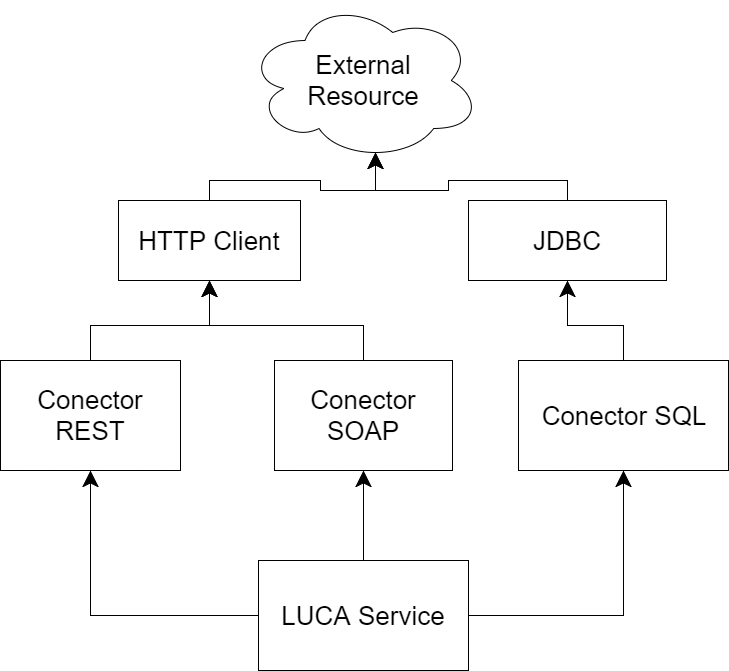
\includegraphics[scale=0.5]{conectorImplementation.png}
	\caption{Arquitectura del Conector}\label{fig:conectorImplementation}
\end{figure}

\subsection{Arquitectura del Process-Component}

El Process-Component es un proyecto abstracto (debe de ser importado e implementado por un proyecto o componente padre) encargado de recibir y comunicar los eventos realizados sobre una interfaz construida a partir de la librería GO.JS.

\vspace{5mm}

La arquitectura del Process-Component se ostenta en dos pilares. El primero es la implementación de la lógica del propio componente y el segundo es la implementación de un conector que se comunica con una librería de GO.JS que también debe de ser definida.

\vspace{5mm}

La lógica del componente se basa en un estado ( el cuál alberga todos los elementos para poder formar la vista), y en una serie de acciones o comandos que se pueden realizar sobre él, y donde tras cada acción, se realiza una comunicación con el conector para que este se encargue de modificar el estado de los elementos de GO.JS.

\vspace{5mm}

El conector internamente se compone de la librería encargada de definir el ámbito gráfico con el que se va a trabajar, de una serie de eventos que serán trasladados a la lógica del Process-Component, y de modificar los elementos en activo en la vista bajo la orden especificada.

\vspace{5mm}

A continuación, se muestra una figura explicativa de dicha interacción interna entre los componentes:

\begin{figure}[H]
	\centering
	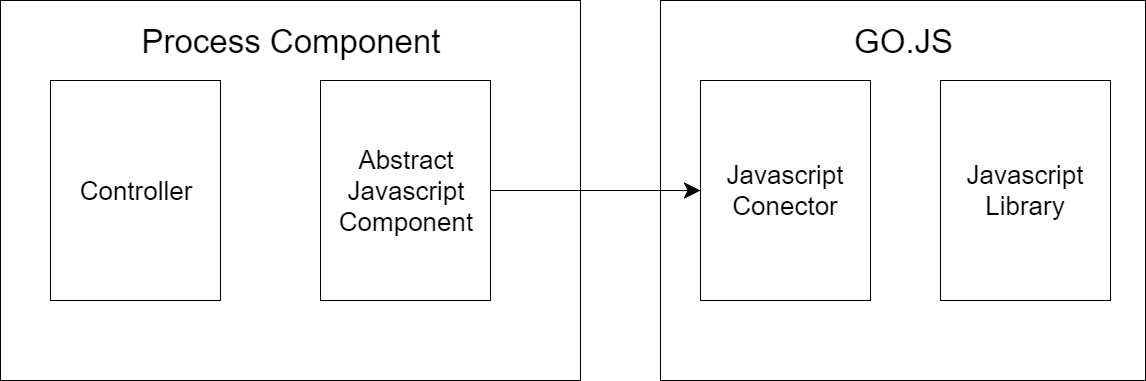
\includegraphics[scale=0.5]{processComponentArquitectura.png}
	\caption{Arquitectura del Process-Component}\label{fig:processComponent}
\end{figure}

Como resumen del funcionamiento del Process-Component, éste es el encargado de recibir eventos realizados sobre la interfaz gráfica, a través del conector hasta llegar a la lógica del componente para publicarlos o abstraerlos a un conjunto de elementos escuchadores que deberán de ser atendidos por el componente implementador de este Process-Component.


\section{Planificación}


	La sección presente describe el proceso llevado a cabo para realizar la implementación tanto del componente gráfico (Process-Component) como del componente de Luca (Luca-Process).

	\vspace{5mm}

	El proceso que se llevó a cabo para realizar el desarrollo del proyecto se basó en dos fases:
	
	\begin{itemize}
		\item  Una primera en la que se estudió el funcionamiento de la herramienta gráfica de GO.JS y después se realizó la implementación del Process-Componet.
		\item  Una segunda en la que utilizando el componente descrito anteriormente, se implementa un incremento utilizando la lógica previa de LUCA.

	\end{itemize}

\subsection{Implementación}
	A continuación se explica brevemente el proceso de implementación llevado a cabo para ambas fases:
	\begin{itemize}
		\item Process-Component
			\subitem El primer paso para empezar la implementación del Process-Component, fue aprender y practicar con ejemplos y con pruebas de concepto para ver como funcionaba y aprender la sintaxis de la librería de GO.JS.
			
			\vspace{5mm}
			
			Tras este primer paso, se realizó la implementación del modelo (se puede encontrar en los documentos técnicos), para posteriormente generar una primera prueba de concepto conjunta realizando una comunicación con la librería GO.JS.
			
			
			\vspace{5mm}
			
			Por último se implementaron los eventos y escuchadores para posteriormente centrarse en completar dicho componente.
			
			
			
		\item  Luca-Process
			\subitem En este componente se sigue un metodología similar al anterior. Primero se crea una prueba de concepto sencilla para ver la comunicación entre los componentes para posteriormente empezar a montar todo el sistema de recepción de eventos y llamadas al componente gráfico.
			
			\vspace{5mm}
			
			El siguiente paso fue seguir el estilo arquitectónico ya existente en LUCA, utilizando el patrón MVP\cite{mvp} para crear toda la jerarquíca de capas necesarias para la comunicación con los servicios ya existentes de LUCA y la propia base de datos de LUCA.
		
	\end{itemize}

	
\subsection{Pruebas}

	Este apartado describe el proceso de pruebas llevado a cabo para la comprobación y verificación de las diferentes funcionalidades del proyecto.
	
	\vspace{5mm}
	
	Las pruebas se centraron principalmente en el Luca-Process, ya que es el componente que alberga la mayor lógica del proyecto debido al conjunto de servicios que lo compone y a la lógica sobre los presenters desplegada.
	
	\vspace{5mm}
	
	Profundizando en las pruebas implementadas, solo se han realizado pruebas de integración por varios motivos. El primero es que las pruebas unitarias no son necesarias hacerlas ya que se centran sobre la capa de repositorio y esta capa ha sido implementada con Spring Data Jpa\cite{jpa} y ofrece ya una fiabilidad. El motivo por el que no se realizaron pruebas de sistema, aunque en una primera planificación estaban previstas hacerlas integrandolas con Selenium\cite{selenium} fue la complejidad que lleva la integración junto con Vaadin\cite{vaadin}, ya que la ventaja de programar mediante una captura de eventos sobre la vista toda la secuencia de movimiento sobre dicha vista pasa a ser programática, y debido a que había que ceñirse a unas fechas de entrega y al tiempo que llevaría dicha implementación se decidió omitirlas.
	
	\vspace{5mm}
	
	Las pruebas de integración que se llevaron a cabo se implementaron con Spring Test\cite{springTest} y JUnit\cite{junit}. Desglosando la composición de los mismos, se utilizó en cada test un fichero sql que declaraba las instrucciones de inserción de datos en la base de datos de pruebas necesarios para el correcto funcionamiento de los mismos. La base de datos de pruebas es una base de datos Mysql en local. relacional 
 




	 